\section{局部存在}
\label{sec:odeex-local-existence}

给定一个开集$\bm{D}\subseteq\mathbb{R}\times\mathbb{R}^{n}$、一个连续映射$\bm{f}:\bm{D}\to\mathbb{R}^{n}$和一点$(t_0,\bm{x}_0)\in\bm{D}$，我们要找区间$I\ni t_0$上的连续可微曲线$\bm{x}$，使$(t,\bm{x}(t))\in\bm{D}$，并且
\begin{equation}
 \dot{\bm{x}}(t)=\bm{f}(t,\bm{x}(t)),\quad t\in I,\qquad \bm{x}(t_0)=\bm{x}_0.
 \label{eq:odeex-ivp}
\end{equation}
这样的曲线称为经典解。右端连续时，由第~\ref{chap:ordinary-differential-equations}章的讨论，式~\eqref{eq:odeex-ivp}等价于连续曲线满足积分方程
\begin{equation}
 \bm{x}(t)=\bm{x}_0+\int_{t_0}^{t}\bm{f}(s,\bm{x}(s))\,\mathrm{d}s,\quad t\in I.
 \label{eq:odeex-integral}
\end{equation}
积分号里的被积函数连续，所以满足式~\eqref{eq:odeex-integral}的连续曲线自动连续可微，并且在$t_0$处取值$\bm{x}_0$。

只知道右端连续，能否断定这样的曲线至少存在一小段？图像上的问题是：平面每一点都标着一个小箭头，从起点出发能不能画一条处处与箭头相切的曲线。最自然的办法是顺着箭头走一小步，停下来看新位置的箭头，再走一小步。

\paragraph{顺着方向场走折线}
取步长$h>0$，时间网格$t_k=t_0+kh$。从$\bm{x}^{(0)}=\bm{x}_0$出发，每一步沿当前箭头走直线：
\begin{equation}
 \bm{x}^{(k+1)}=\bm{x}^{(k)}+h\,\bm{f}(t_k,\bm{x}^{(k)}).
 \label{eq:odeex-euler-node}
\end{equation}
把相邻的点用线段连起来，得到一条折线，称为\term{Euler折线}（Euler polygon）。第~\ref{chap:ode-numerical-methods}章会把它当作数值方法研究误差，这里只用它来证明解的存在。

用$\dot x=x^2$，$x(0)=1$在$[0,1/4]$上试算。取$N=2$步，$h=1/8$，两步的结果分别是
\[
 x^{(1)}=1+\frac18\cdot1^2=1.125,\qquad x^{(2)}=1.125+\frac18\cdot1.125^2\approx1.2832.
\]
真解在$t=1/4$处等于$4/3\approx1.3333$。取$N=4$和$N=8$，折线的终点依次为
\[
 1.3053,\qquad 1.3184.
\]
图~\ref{fig:odeex-euler-refinement}画出了这些折线。每条折线都在真解下方，因为$x^2$沿解递增，折线在每段上采用的是该段开始时较小的斜率；步长减半时，折线向真解靠拢。

\begin{BookInlineFigure}
  \centering
  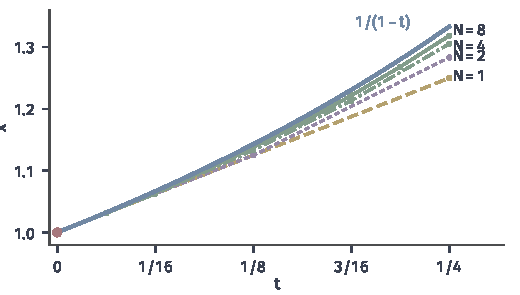
\includegraphics[width=88mm]{figures/06-differential-equations/01-ordinary-differential-equations/matplotlib/odeex-euler-refinement/figure.pdf}
  \caption{初值问题$\dot x=x^2$，$x(0)=1$在$[0,1/4]$上的Euler折线。蓝色粗线是真解$1/(1-t)$，其余折线的步数$N$分别为$1,2,4,8$，红点是初值。步数增加时折线向真解靠拢。}
  \label{fig:odeex-euler-refinement}
\end{BookInlineFigure}

这里的真解是预先知道的。对一般的连续右端，没有真解可作比较，也无从知道折线列是否收敛。我们手里只有折线本身的信息，要从中取出一条极限曲线，就要先把折线关在一个固定的范围内。

\paragraph{盒子与时间窗}
先选一个以初值为中心的盒子。取$a,b>0$足够小，记
\begin{equation}
 \bm{B}_b=\{\bm{x}\in\mathbb{R}^{n}:\lVert\bm{x}-\bm{x}_0\rVert_2\leq b\},\qquad
 \bm{Q}=[t_0-a,t_0+a]\times\bm{B}_b,
 \label{eq:odeex-box}
\end{equation}
使$\bm{Q}\subseteq\bm{D}$。$\bm{D}$是开集，这总能做到。$\bm{Q}$是紧集，连续函数$\lVert\bm{f}\rVert_2$在其上有最大值，取$M>0$使$\lVert\bm{f}\rVert_2\leq M$在$\bm{Q}$上成立。

$M$是盒子内箭头的最大速度。一条曲线只要还在盒子内，到初值的距离就至多以速率$M$增长，所以它被限制在以$(t_0,\bm{x}_0)$为顶点、斜率$\pm M$的锥内。它可能从盒子的上下壁离开，这要花至少$b/M$的时间；也可能走到盒子的左右壁，这要花时间$a$。于是在时间窗
\begin{equation}
 \delta=\min\Bigl\{a,\frac{b}{M}\Bigr\}
 \label{eq:odeex-peano-window}
\end{equation}
内，曲线不会离开盒子。

图~\ref{fig:odeex-existence-box}用前面的方程演示这一计算。取$b=1$，状态范围是$[0,2]$，其上$x^2\leq4$，所以$M=4$。图(a)中$a=1/2$，$\delta=\min\{1/2,1/4\}=1/4$，锥先碰到上壁。图(b)中$a=3/20$，$\delta=3/20$，锥先碰到右壁。真解实际能走到$t=1$，时间窗只是一个保守的保证。

\begin{BookInlineFigure}
  \centering
  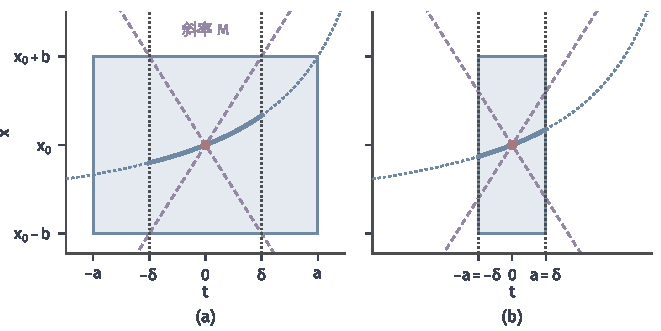
\includegraphics[width=112mm]{figures/06-differential-equations/01-ordinary-differential-equations/matplotlib/odeex-existence-box/figure.pdf}
  \caption{盒子与时间窗。浅蓝矩形是$\bm{Q}$，这里$x_0=1$，$b=1$，紫色虚线是斜率$\pm M=\pm4$的锥，蓝色粗线是真解在时间窗内的部分，蓝色点线是它在窗外的延续。(a)$a=1/2$，$\delta=b/M=1/4$，由状态范围决定。(b)$a=3/20$，$\delta=a$，由时间范围决定。}
  \label{fig:odeex-existence-box}
\end{BookInlineFigure}

\paragraph{Peano存在定理}
盒子内的折线有共同的速度上限，这件事足以让我们从折线列中抽出一条收敛的曲线。结论是下面的\term{Peano存在定理}（Peano existence theorem）。

\begin{theorem}[Peano存在定理]
\label{thm:odeex-peano}
设$\bm{D}\subseteq\mathbb{R}\times\mathbb{R}^{n}$是开集，$\bm{f}:\bm{D}\to\mathbb{R}^{n}$连续，$(t_0,\bm{x}_0)\in\bm{D}$。按式~\eqref{eq:odeex-box}取$\bm{Q}\subseteq\bm{D}$，取$M>0$使$\lVert\bm{f}\rVert_2\leq M$在$\bm{Q}$上成立，再按式~\eqref{eq:odeex-peano-window}确定$\delta$。则初值问题~\eqref{eq:odeex-ivp}在$[t_0-\delta,t_0+\delta]$上至少有一个经典解，解的取值都在$\bm{B}_b$中。
\end{theorem}

证明分三步：折线留在盒子内，折线列有一致收敛的子列，子列的极限满足积分方程。第一步用$\bm{f}$的有界性，第二步用有限维的紧性，第三步用$\bm{f}$的连续性。

\begin{proof}
先在$I^+=[t_0,t_0+\delta]$上构造解。对正整数$N$，取$h=\delta/N$，按式~\eqref{eq:odeex-euler-node}得到节点$\bm{x}^{(0)},\ldots,\bm{x}^{(N)}$，记相应的折线为$\bm{y}_N$，即对$t\in[t_k,t_{k+1}]$，
\[
 \bm{y}_N(t)=\bm{x}^{(k)}+(t-t_k)\,\bm{f}(t_k,\bm{x}^{(k)}).
\]

\emph{折线留在盒子内。}对$k$归纳证明$\lVert\bm{x}^{(k)}-\bm{x}_0\rVert_2\leq Mkh$。$k=0$时成立。若对$k<N$成立，则$Mkh\leq M\delta\leq b$，$(t_k,\bm{x}^{(k)})\in\bm{Q}$，所以$\lVert\bm{f}(t_k,\bm{x}^{(k)})\rVert_2\leq M$，于是
\[
 \lVert\bm{x}^{(k+1)}-\bm{x}_0\rVert_2\leq\lVert\bm{x}^{(k)}-\bm{x}_0\rVert_2+hM\leq M(k+1)h.
\]
因此所有节点都在球$\bm{B}_b$中。球是凸集，线段也在其中，折线的取值全在$\bm{B}_b$内，节点上的速度都不超过$M$。

\emph{抽取收敛子列。}折线每段的斜率范数不超过$M$，所以对$s,t\in I^+$，
\[
 \lVert\bm{y}_N(t)-\bm{y}_N(s)\rVert_2\leq M\lvert t-s\rvert.
\]
这说明$\{\bm{y}_N\}$的各分量等度连续，而它们又一致有界（取值在$\bm{B}_b$中）。紧区间上一致有界且等度连续的实函数族，由Arzelà--Ascoli判据在一致距离下相对紧，每个序列都有一致收敛的子列，可参考\BookChapterRef{chap:function-class-covers}{卷四第13章“函数类的有限覆盖”}。对$n$个分量依次抽取子列，得到$\bm{y}_{N_j}$一致收敛到连续曲线$\bm{x}:I^+\to\bm{B}_b$。

\emph{极限满足积分方程。}对$s\in[t_k,t_{k+1})$，记$\sigma_N(s)=t_k$，它是$s$所在网格段的左端点。折线分段线性，由其构造，
\[
 \bm{y}_N(t)=\bm{x}_0+\int_{t_0}^{t}\bm{f}\bigl(\sigma_N(s),\bm{y}_N(\sigma_N(s))\bigr)\,\mathrm{d}s.
\]
$\bm{f}$在紧集$\bm{Q}$上一致连续。任取$\varepsilon>0$，存在$\eta>0$，使$\bm{Q}$中两点的时间差与状态距离之和小于$\eta$时，$\bm{f}$值之差的范数小于$\varepsilon$。

比较被积函数在两点的取值：时间差是$s-\sigma_N(s)\leq h$，状态差由三角不等式与斜率上限满足
\[
 \lVert\bm{y}_N(\sigma_N(s))-\bm{x}(s)\rVert_2\leq Mh+\lVert\bm{y}_N-\bm{x}\rVert_{\infty},
\]
这里$\lVert\cdot\rVert_{\infty}$是$I^+$上的一致范数。沿子列$N=N_j$，$h\to0$，$\lVert\bm{y}_N-\bm{x}\rVert_{\infty}\to0$，所以当$j$足够大时，两点距离之和小于$\eta$，对所有$s$都有被积函数之差小于$\varepsilon$。

积分后得到，对$t\in I^+$，
\[
 \Bigl\lVert\int_{t_0}^{t}\bm{f}\bigl(\sigma_N(s),\bm{y}_N(\sigma_N(s))\bigr)\,\mathrm{d}s
 -\int_{t_0}^{t}\bm{f}(s,\bm{x}(s))\,\mathrm{d}s\Bigr\rVert_2\leq\varepsilon\delta.
\]
令$j\to\infty$，$\bm{x}$在$I^+$上满足积分方程~\eqref{eq:odeex-integral}。

\emph{向左延伸。}令$\tilde{\bm{x}}(s)=\bm{x}(2t_0-s)$，方程变成
\[
 \frac{\mathrm{d}\tilde{\bm{x}}}{\mathrm{d}s}=-\bm{f}(2t_0-s,\tilde{\bm{x}}),
\]
其右端满足同样的条件和同样的上界。对它应用前面的结论，得到$[t_0-\delta,t_0]$上的解。两段在$t_0$处都取$\bm{x}_0$，合起来在整个区间上满足式~\eqref{eq:odeex-integral}，因而是经典解。
\end{proof}

\paragraph{连续性在哪里起作用}
证明第三步用连续性把折线所用的箭头换成极限曲线上的箭头。若右端不连续，这一步会失败，解也可能真的不存在。取
\[
 f(x)=\begin{cases}-1,&x\geq0,\\ 1,&x<0,\end{cases}\qquad x(0)=0.
\]
箭头从两侧都指向$x=0$，图~\ref{fig:odeex-discontinuous-chatter}(a)中从$x=\pm1$出发的解都在$t=1$到达零线，到达之后就停在那里。

假设有解从$x(0)=0$出发。若解在某段时间内为正，这段时间的左端点处解为零，而解在段内以速度$-1$下降，不可能从$0$变成正数；同理解不能在某段时间内为负。于是解只能恒为零，而$\dot x=0$不等于$f(0)=-1$，矛盾。

Euler折线看到的是什么？在图~\ref{fig:odeex-discontinuous-chatter}(b)中，它在$0$与$-h$之间来回跳动，当$h\to0$时一致收敛到$x\equiv0$。折线列本身有极限，但折线所用的斜率在$\pm1$之间振荡，平均为$0$，而$f(0)=-1$。极限曲线不满足方程，正是因为第三步的“被积函数收敛”不成立。

\begin{BookInlineFigure}
  \centering
  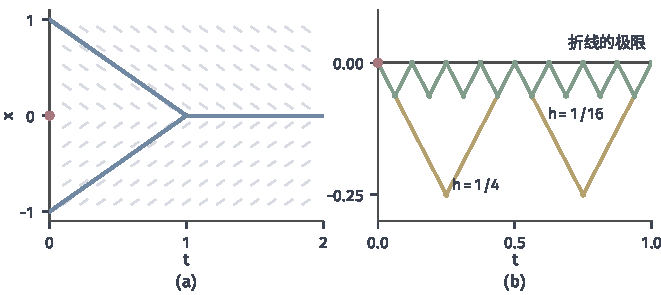
\includegraphics[width=112mm]{figures/06-differential-equations/01-ordinary-differential-equations/matplotlib/odeex-discontinuous-chatter/figure.pdf}
  \caption{右端不连续时存在性失败。$f(x)=-1$（$x\geq0$），$f(x)=1$（$x<0$）。(a)短线是方向场，蓝线是从$x=\pm1$出发的解，到$t=1$时汇入零线后停止延伸，红点是无解的初值$(0,0)$。(b)从红点出发的两条Euler折线，黄线$h=1/4$，绿线$h=1/16$，$h\to0$时一致趋于灰线$x\equiv0$，该极限不是解。}
  \label{fig:odeex-discontinuous-chatter}
\end{BookInlineFigure}

\paragraph{连续不保证唯一}
定理~\ref{thm:odeex-peano}说“至少一个”，这个说法不能加强。考虑
\begin{equation}
 \dot x=2\sqrt{\lvert x\rvert},\qquad x(0)=0.
 \label{eq:odeex-sqrt}
\end{equation}
右端处处连续。$x\equiv0$代入后两端都是零，成立。对$x=t^2$（$t\geq0$），左端$2t$，右端$2\sqrt{t^2}=2t$，也成立。

不止这两条。对每个$c\geq0$，定义
\[
 x_c(t)=\begin{cases}0,&t\leq c,\\(t-c)^2,&t>c.\end{cases}
\]
在$t>c$时验证与刚才相同，在$t=c$处左右导数都是$0$，等于右端的值，所以$x_c$是经典解。解可以在零线上停留任意长的时间，然后在任意时刻起飞。图~\ref{fig:odeex-sqrt-funnel}画出了这束解，它们从同一个红点出发，初值完全相同，将来却不同。

\begin{BookInlineFigure}
  \centering
  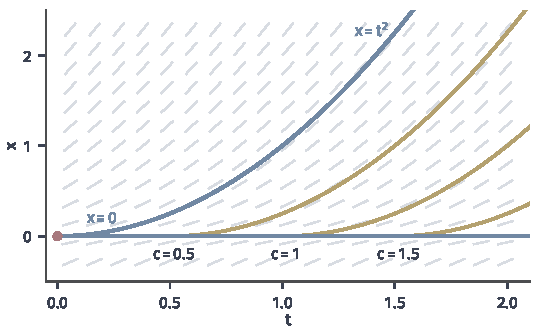
\includegraphics[width=92mm]{figures/06-differential-equations/01-ordinary-differential-equations/matplotlib/odeex-sqrt-funnel/figure.pdf}
  \caption{初值问题~\eqref{eq:odeex-sqrt}的多个解。短线是方向场，红点是初值$(0,0)$。蓝线是$x\equiv0$与$x=t^2$，黄线是在$t=c$时离开零线的解$x_c$，$c=0.5,1,1.5$。任意$c\geq0$都给出一条解。}
  \label{fig:odeex-sqrt-funnel}
\end{BookInlineFigure}

为什么连续性不足以挑出一条解？$x$接近$0$时，箭头斜率$2\sqrt{\lvert x\rvert}$相对于$\lvert x\rvert$大得不成比例：比值$2/\sqrt{\lvert x\rvert}$趋于无穷。于是离开零线一点点就有足够的速度继续远离，离开零线并不需要一个有限的“推力”。

多解还解释了为什么证明中要抽子列。考虑方程
\[
 \dot x=2\operatorname{sgn}(x)\sqrt{\lvert x\rvert},\qquad x(0)=0,
\]
它同样有解$x\equiv0$和$x=\pm t^2$。若折线的初值恰好是$0$，它恒为零；但若初值带一个微小的扰动$x^{(0)}=(-1)^N/N^2$，比如计算时的舍入，$N$为偶数和奇数时折线会走向不同的解。

取$N$为偶数，步长$h=\delta/N$，其中$\delta=1$。令$s_k=\sqrt{x^{(k)}}$，由式~\eqref{eq:odeex-euler-node}，
\[
 s_{k+1}^2=s_k^2+2hs_k.
\]
当$s_k\geq h/4$时，$(s_k+h/2)^2=s_k^2+hs_k+h^2/4\leq s_k^2+2hs_k$，所以$s_{k+1}\geq s_k+h/2$。而$s_0=1/N=h$，于是对所有$k$，
\[
 x^{(k)}\geq\bigl(s_0+kh/2\bigr)^2\geq\Bigl(\frac{t_k}{2}\Bigr)^2.
\]

奇数$N$的折线是偶数情形的镜像。所以偶数列的极限至少是$t^2/4$，奇数列的极限至多是$-t^2/4$，整列折线没有极限，如图~\ref{fig:odeex-odd-sqrt-euler}所示。紧性只给出“有收敛的子列”，不同子列可以收敛到不同的解。

\begin{BookInlineFigure}
  \centering
  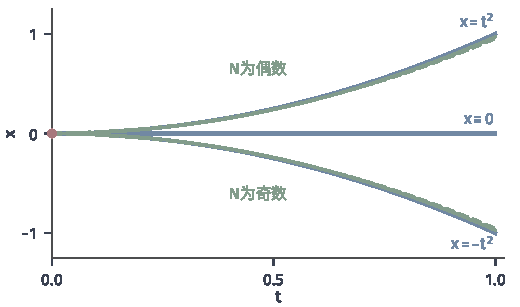
\includegraphics[width=88mm]{figures/06-differential-equations/01-ordinary-differential-equations/matplotlib/odeex-odd-sqrt-euler/figure.pdf}
  \caption{$\dot x=2\operatorname{sgn}(x)\sqrt{\lvert x\rvert}$的Euler折线，初值$x^{(0)}=(-1)^N/N^2$，步长$1/N$。绿色虚线$N=20,21$，绿色实线$N=80,81$，蓝线是从$(0,0)$出发的三条解。偶数$N$贴近$t^2$，奇数$N$贴近$-t^2$，整列不收敛。}
  \label{fig:odeex-odd-sqrt-euler}
\end{BookInlineFigure}

\paragraph{紧性只属于有限维}
证明的第二步用了“一致有界且等度连续的曲线族相对紧”。它的前提是每个时刻的取值落在一个紧集中，而$\mathbb{R}^{n}$的闭球恰好是紧的。在无限维空间中闭球不紧，这一步不能照搬，结论也确实会失败。

设$c_0$是收敛到零的实数列$\bm{x}=(x_1,x_2,\ldots)$组成的空间，范数取各坐标绝对值的上确界，记为$\lVert\bm{x}\rVert_{\infty}$，它是完备的。定义$\bm{f}:c_0\to c_0$，
\[
 \bigl(\bm{f}(\bm{x})\bigr)_n=2\sqrt{\lvert x_n\rvert}+\frac{1}{n+1},\qquad n\geq1.
\]
第一项随$n\to\infty$趋于零，第二项也是，所以$\bm{f}(\bm{x})\in c_0$。对实数$a,b$，有
\[
 \lvert\sqrt{\lvert a\rvert}-\sqrt{\lvert b\rvert}\rvert\leq\sqrt{\lvert a-b\rvert}.
\]
逐坐标使用它，得到
\[
 \lVert\bm{f}(\bm{x})-\bm{f}(\bm{y})\rVert_{\infty}\leq2\sqrt{\lVert\bm{x}-\bm{y}\rVert_{\infty}},
\]
所以$\bm{f}$连续。

假设$\bm{x}(t)$是$[0,\delta)$上取值于$c_0$的解，$\bm{x}(0)=\bm{0}$。在范数下可微蕴含每个坐标可微，所以每个坐标满足$\dot x_n=2\sqrt{\lvert x_n\rvert}+1/(n+1)>0$。于是$x_n(t)>0$对$t>0$成立，并且
\[
 \frac{\mathrm{d}}{\mathrm{d}t}\sqrt{x_n}=\frac{\dot x_n}{2\sqrt{x_n}}\geq1.
\]
从$s>0$积分到$t$，再令$s\downarrow0$，得到$\sqrt{x_n(t)}\geq t$，即对所有$n$，
\[
 x_n(t)\geq t^2.
\]
每个坐标都不低于同一个正数，这与$\bm{x}(t)\in c_0$矛盾。因此这个连续方程在$c_0$中没有解。

图~\ref{fig:odeex-c0-coordinates}算出了各坐标的实际取值。右端的序列在$t=0$时衰减，解的坐标却被$t^2$托住，在任何$t>0$时都不再衰减到零。$\bm{f}$的连续性和局部有界性都在，只是缺了紧性。

\begin{BookInlineFigure}
  \centering
  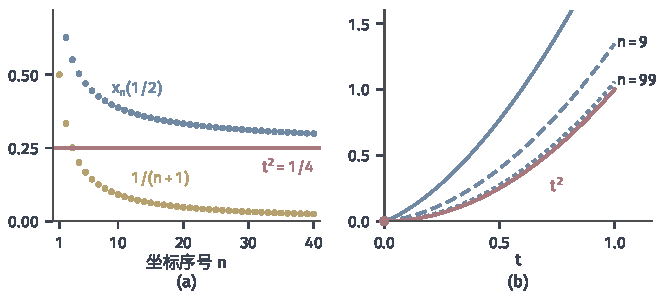
\includegraphics[width=112mm]{figures/06-differential-equations/01-ordinary-differential-equations/matplotlib/odeex-c0-coordinates/figure.pdf}
  \caption{$c_0$中无解方程的坐标。各坐标单独满足$\dot x_n=2\sqrt{x_n}+1/(n+1)$，$x_n(0)=0$，由数值积分算出。(a)$t=1/2$时的取值，蓝点$x_n(1/2)$都在红线$t^2=1/4$之上，黄点$1/(n+1)$是右端在$t=0$的序列。(b)蓝线为$n=1,9,99$时的$x_n(t)$，都在红线$t^2$之上，$n$增大时趋于$t^2$而不趋于$0$。}
  \label{fig:odeex-c0-coordinates}
\end{BookInlineFigure}
